\documentclass[25pt,landscape]{tikzposter}
\usepackage[utf8]{inputenc}
\usepackage{multicol}
\usepackage{xcolor}
\usepackage{blindtext}
\usepackage{comment}
\usepackage{adjustbox}

\title{Clasificación de Textos: Naive Bayes vs Neural Networks}
\author{David Pérez Gómez \& Guzmán López Santamaría}
\date{}
\institute{EUITI - UPV/EHU}

\usetheme{Desert}
\usecolorstyle{Denmark}

\tikzposterlatexaffectionproofoff

\settitle{ \centering \vbox{
\centering
\color{white} {\bfseries \Huge \sc \@title \par}
\vspace*{1em}
{\huge \@author \par} \vspace*{1em} {\LARGE \@institute}
}}


\begin{document}

\maketitle
\begin{columns}
	\column{0.30}
	\block{OBJETIVOS}{
	\paragraph{}Dado un conjunto de datos de autopsias verbales se quiere realizar un proceso de clasificación mediante el cual se prediga una clase para cada instancia. Este proceso se llevará a cabo mediante dos clasificadores diferentes y representando el conjunto de datos de dos formas distintas. El objetivo de este proyecto es analizar y comparar los resultados obtenidos para cada uno de los clasificadores y de las representaciones.
	}
	
	\column{0.70}
	\block{DATOS}{
	\begin{minipage}[t]{0.45\linewidth}
	\paragraph{}El conjunto de datos es Verbal Autopsies, un conjunto de autopsias verbales realizadas en diversos países y que agrupa una gran variedad de enfermedades y causas de muerte. Serán estas las que nuestro clasificador utilice como clase a predecir. En cuanto a las entradas, utilizaremos el atributo correspondiente a la autopsia verbal en sí (gs\_text34).
	\paragraph{}A estos datos se les ha de aplicar un preproceso previo, pues usar los datos tal y como los hemos obtenido no es lo más óptimo para nuestro proceso de representación y clasificación. En la siguiente tabla se aparece orden de las operaciones de preproceso:

	\end{minipage}
	\begin{adjustbox}{valign=t}
	\begin{minipage}[t]{0.2\linewidth}
	\end{minipage}
	 \textcolor{white}{XD} %No borrar, hace que haya división entre las minipage
	\end{adjustbox}
	\begin{adjustbox}{valign=t}
	\begin{minipage}[t]{0.3\linewidth}
	\begin{tikzfigure}
	\begin{tabular}{|l|l|}
	\hline
	\textbf{Flujo de cambios} & \textbf{Descripción} \\ \hline
	Raw 					& Conjunyo de textos original. \\
	Limpieza textos vacíos 	& Se eliminan manualmente instancias duplicadas y aquellas que están vacías.\\
	Tokenizer 				& Se eliminan las palabras que no aportan información (artículos, etc.).\\
	Minusculas 				& Se convierte todo el texto a letras minúsculas. \\
	Stemmer 				& Se sustituye cada palabra por su raíz. \\ \hline
	\end{tabular}
	\end{tikzfigure}
	\end{minipage}\\
	\end{adjustbox}
	}	
\end{columns}	

\begin{columns}
	\column{0.30}
	\block{REPRESENTACIÓN DE TEXTOS}{ }
    \block{TF-IDF}{
    	\paragraph{}TF-IDF es una medida estadística que sirve para calcular la importancia de una palabra dentro de un texto. De forma simplificada, se considera que la importancia de una palabra aumenta cuantas más apariciones tenga en un documento dado, pero a su vez es inversamente proporcional a su ratio de aparición en otros documentos.
    }
    \block{Document Embeddings}{
		\paragraph{}Mediante Document Embeddings se puede representar cada texto de un conjunto de estos como un vector con valores numéricos. Sin embargo, al contrario que TF-IDF, Document Embeddings no crea un vector con tantos valores como palabras en el vocabulario, sino que se trata de un modelo que se entrena con un conjunto de textos y después, es capaz de asignar a nuevos textos vectores de forma que cuanto más similares sean dos textos, más cercanos serán sus correspondientes vectores.
		\paragraph{}En nuestro caso utilizamos la librería Gensim para hacer esta transformación.
    }
    \column{0.30}
   	\block{CLASIFICADORES}{}
	\block{Naive Bayes}{
		\paragraph{}Como clasificador de referencia hemos decidido utilizar Naive Bayes. Este algoritmo calcula la probabilidad de pertenencia a cada clase para cada atributo en función de su valor. Con esto se está suponiendo que los atributos son independientes entre sí. Cuando se dispone a clasificar, realiza la predicción en función de las probabilidades calculadas para cada uno de los atributos de la instancia dada y selecciona la clase que maximice esta probabilidad.
		\paragraph{}Debido a que Naive Bayes asume una total independencia entre clases, consideramos que este clasificador es una buena base para comparar con otro clasificador más complejo.
    }
    \block{Redes Neuronales}{
		\paragraph{}Como clasificador avanzado decidimos utilizar un clasificador combinado formado por varias instancias de Multilayer Perceptron. El Multilayer Perceptron es una red neuronal compuesta por perceptrones (neuronas) y pesos sinápticos conectados entre sí. Recibe una serie de atributos como inputs con los que genera el output. Comparando el output generado con el esperado, el modelo aprende actualizando los pesos sinápticos según corresponda.
		\paragraph{}Para nuestra implementación utilizamos un número de clasificadores Multilayer Perceptron, todos con el mísmo número de neuronas y de capas ocultas, pero entrenados con conjuntos de datos ligeramente distintos, obtenidos aplicando bootstrapping al conjunto de entrenamiento original. Después del entrenamiento, se obtiene la acuracy de cada clasificador al predecir el conjunto de entrenamiento original. Para predecir, se calcula la media ponderada de las probabilidades dadas por cada modelo en función de la accuracy que se le asignó a cada uno y se escoge la clase con mayor probabilidad.
    }

    \column{0.40}
    \block{RESULTADOS}{
    	\paragraph{}Los resultados se han obtenido aplicando el método 10-fold cross-validation a cada modelo utilizando los dos métodos de representación de atributos. En el caso del modelo de redes neuronales, realizamos distintas pruebas, cambiando los paŕametros (nº de modelos, nº de capas ocultas, nº de neuronas) y nos quedamos con los mejores resultados obtenidos.
    	\paragraph{}Los resultados muestran, por un lado, que nuestro modelo tiene ligeramente más éxito que el de referencia, independientemente de la representación usada. También se puede ver que la decisión de utilizar TF-IDF para representar los atributos o de utilizar Document Embeddings también afecta al resultado, obteniendose méjores resultados con TF-IDF en ambos clasificadores. Es muy posible que al crear vectores de tamaño considerablemente menor, con Document Embeddings se pierda bastante información, lo que cause los peores resultados.
		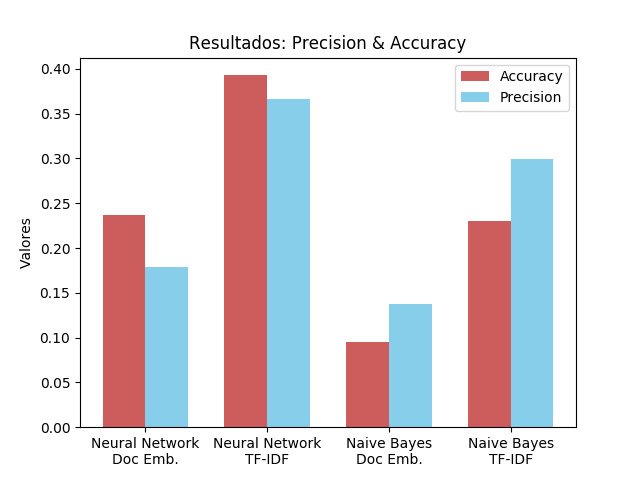
\includegraphics[scale=1.9]{img/PrecisionAccuracy.jpeg}
    }
    
\end{columns}
 	
\end{document}